\chapter{L'analisi delle funzionalità}

La realizzazione di qualunque prodotto software inizia da una fase in cui,
partendo dall’abstract del progetto, si analizzano i requisiti e le funzionalità da realizzare.
L’obiettivo è arrivare ad una definizione delle proprietà e
del comportamento desiderato nell’applicazione che sia concisa e condivisa col cliente,
senza però entrare nel merito delle scelte implementative.\\
Solo a quel punto si può procedere con lo sviluppo del programma vero e proprio.\\
\\
L'abstract del progetto è il seguente:\\
\\
Wyd è un'applicazione che permette ai clienti di organizzare i propri impegni,
siano essi confermati oppure proposti.
Mette a disposizione due calendari,
il primo con gli eventi in cui l'utente è convinto di partecipare,
il secondo in cui vengono riuniti gli eventi a cui l'utente è stato invitato ma senza aver ancora dato conferma.
L'utente ha la possibilità di creare, modficare, confermare o disdire un evento,
ma anche condividerlo con altri o allegarci foto.\\
\\
La condivisione di un evento può avvenire con applicazioni esterne tramite la generazione di un link o
grazie all'ausilio di gruppi di profili.
Inoltre, al termine di un evento, l'applicazione carica automaticamente le foto scattate
durante l'evento, per allegarle a seguito della conferma dell'utente.
L'utente può infatti cercare altri profili e creare gruppi con i profili trovati.
Tutta l'interazione avviene tramite l'utilizzo di profili,
che permettono di suddividere semanticamente gli eventi e le relazioni.
\clearpage

\section{L'individuazione dei requisiti e dei casi d’uso}

Lo studio dell’abstract del progetto porta all’individuazione e
alla descrizione delle sue caratteristiche essenziali.
In particolare, si distinguono i requisiti ed i casi d'uso.
I requisiti formalizzano le funzionalità che l'applicazione deve fornire,
sintetizzando e schematizzando le parti che descrivono del prodotto.
I casi d'uso descrivono invece le interazioni previste tra l'utente e il sistema,
suddividendo le funzionalità in azioni elementari.\\
\subsection{I requisiti e il vocabolario}
I requisiti devono risultare chiari e precisi
per permettere di procedere alle fasi sucessive in maniera corretta e trasparente.
Ogni requisito deve essere breve e puntuale, limitato ad un solo particolare desiderata,
focalizzando una necessità specifica.\\
\\
Si suddividono in funzionali o non funzionali in base alle loro caratteristiche.\\
I requisiti funzionali descrivono le funzionalità che il sistema deve fornire,
mentre i requisiti non funzionali illustrano le caratteristiche che il sistema deve soddisfare per essere considerato valido.\\

Si noti come le caratteristiche di velocità e scalabilità vengono individuate ed introdotte fin da subito.
\begin{longtable} {|P{1.3cm}|P{11.2cm}|P{3cm}|}
    \hline
    \textbf{ID} & \textbf{Requisiti}                                                          & \textbf{Tipo}  \\
    \hline
    R1F         & Registrazione di un account tramite l’interfaccia web                       & Funzionale     \\
    \hline
    R2F         & Identificazione attraverso mail univoca e password di almeno 6 caratteri    & Funzionale     \\
    \hline
    R3F         & Visualizzazione degli eventi confermati                                     & Funzionale     \\
    \hline
    R4F         & Visualizzazione degli eventi proposti                                       & Funzionale     \\
    \hline
    R5F         & Creazione di un evento impostando almeno la data di inizio e quella di fine & Funzionale     \\
    \hline
    R6F         & La data di fine deve essere successiva alla data di inizio                  & Funzionale     \\
    \hline
    R7F         & Modifica di un evento                                                       & Funzionale     \\
    \hline
    R8F         & La conferma di un evento lo sposta negli eventi confermati                  & Funzionale     \\
    \hline
    R9F         & La disdetta di un evento lo sposta negli eventi proposti                    & Funzionale     \\
    \hline
    R10F        & Caricamento delle foto di un evento                                         & Funzionale     \\
    \hline
    R11F        & Condivisione tramite link                                                   & Funzionale     \\
    \hline
    R12F        & Condivisione tramite gruppo o ad altri profili                              & Funzionale     \\
    \hline
    R13F        & Ricerca automatica delle foto sul dispositivo mobile                        & Funzionale     \\
    \hline
    R14F        & Conferma delle foto                                                         & Funzionale     \\
    \hline
    R15F        & Ricerca di altri profili                                                    & Funzionale     \\
    \hline
    R16F        & Creazione di un gruppo da due o più profili                                 & Funzionale     \\
    \hline
    R17F        & Visualizzazione dei profili collegati                                       & Funzionale     \\
    \hline
    R18F        & Creazione di un nuovo profilo                                               & Funzionale     \\
    \hline
    R19F        & Cambio del profilo attualmente in uso                                       & Funzionale     \\
    \hline
    R20F        & Aggiornamento in tempo reale delle modifiche agli eventi                    & Funzionale     \\
    \hline
    R1NF        & Per interagire l’utente deve essere autenticato                             & Non Funzionale \\
    \hline
    R2NF        & Velocità di richiesta iniziale dei dati                                     & Non Funzionale \\
    \hline
    R3NF        & Semplicità e fluidità dell'interfaccia grafica                              & Non Funzionale \\
    \hline
    R4NF        & Velocità in lettura e scrittura dei dati                                    & Non Funzionale \\
    \hline
    R5NF        & Velocità nella ricerca dei profili                                          & Non Funzionale \\
    \hline
    R6NF        & Scalabilità delle richieste                                                 & Non Funzionale \\
    \hline
    \caption{Tabella dei requisiti di Wyd}
\end{longtable}


Alla tabella dei requisiti si affianca quella del vocabolario,
definendo i termini utilizzati nel progetto per allinearli definitivamente alle volontà del cliente.\\

\begin{longtable} {|P{3.5cm}|P{9cm}|P{3cm}|}
    \hline
    \textbf{Voce}     & \textbf{Definizione}                                                             & \textbf{Sinonimi}                 \\
    \hline
    Account           & combinazione di mail e password che identifica un utente                         &                                   \\
    \hline
    Utente            & Persona che utilizza l’applicazione                                              &                                   \\
    \hline
    Profilo           & Entità logica che raggruppa eventi e interazioni                                 &                                   \\
    \hline
    Profili collegati & Profili a cui l'utente può avere accesso                                         &                                   \\
    \hline
    Gruppo            & Insieme di profili                                                               &                                   \\
    \hline
    Evento            & Azione(o previsione di azione) con una durata nel tempo                          &                                   \\
    \hline
    Data e ora evento & Indicazione temporale del momento in cui avverrà l'azione                        &                                   \\
    \hline
    Evento confermato & Evento a cui il profilo ha dato conferma di partecipazione                       &                                   \\
    \hline
    Evento proposto   & Evento a cui il profilo non ha dato conferma di partecipazione                   & Evento disdetto, evento condiviso \\
    \hline
    Email             & Indirizzo di posta elettronica del cliente utilizzata anche per l'autenticazione &                                   \\
    \hline
    Password          & Codice alfanumerico di almeno 8 caratteri                                        &                                   \\
    \hline
    Credenziali       & Insieme composto da email e password necessari per accedere al sistema           &                                   \\
    \hline
    \caption{Vocabolario di Wyd}
\end{longtable}


\subsection{I casi d’uso}

I casi d’uso descrivono le interazioni tra gli attori ed il sistema, suddividendo le funzionalità in azioni elementari.
Si definiscono attori tutti gli elementi che compiono una parte attiva nei confronti del programma.
Ogni attore può interagire con uno o più casi d'uso,
ed ogni caso d'uso può essere relazionazionato con altri, definendo la loro relazione.\\
\\
I casi d'uso possono essere collegati tra loro tramite rapporti di inclusione o estensione.
Si dice che un caso include un altro se contiene il suo comportamento.
Si dice invece che un caso d'uso ne estende un altro se il suo comportamento può essere inserito all'interno del secondo.\\
\\

\begin{figure}[htb]
    \centering
    \adjustbox{width=\textwidth}{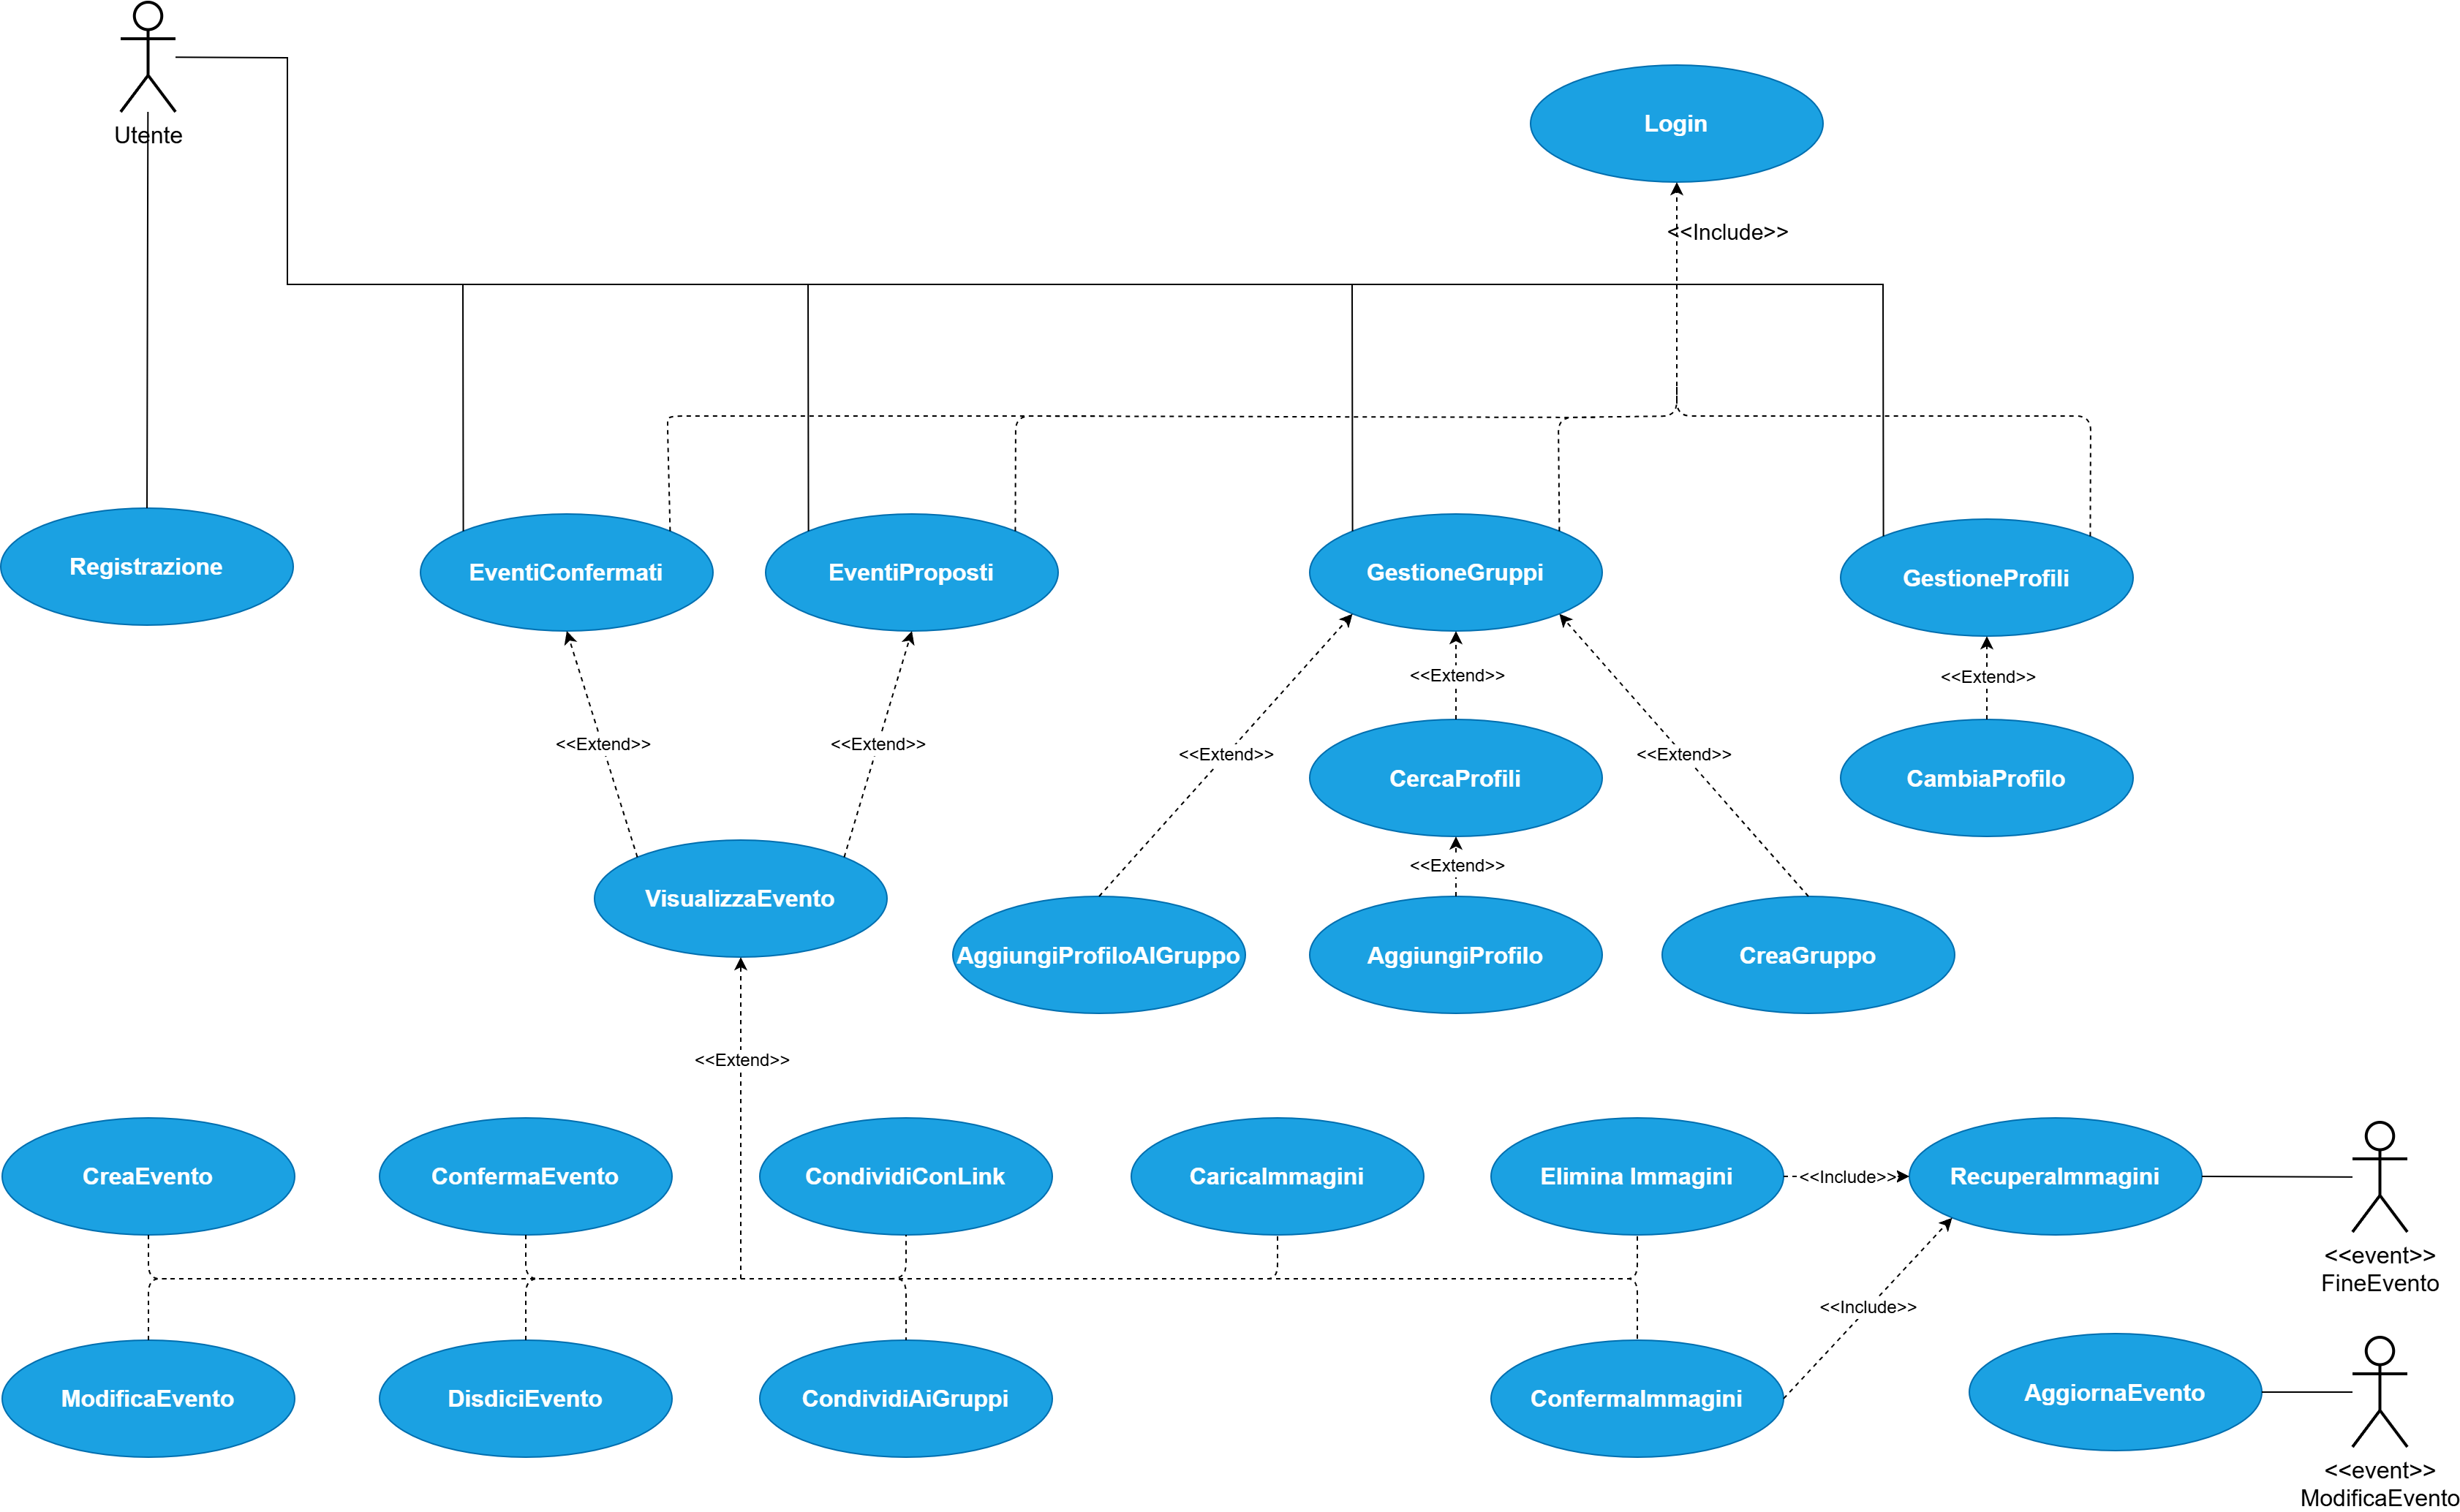
\includegraphics{Casiduso.png}}
    \caption{Diagramma dei casi d'uso}
\end{figure}
\clearpage
Per ogni caso d'uso viene identificato uno scenaro di utilizzo, che chiarifica il contesto, il comportamento ed i punti critici dell'utilizzo.
In particolare, si riportano gli scenari di utilizzo per i principali casi d'uso di Wyd, ovvero quelli
che più andranno ad impattare sulla struttura e sulle esigenze del progetto.\\
\\
Lo scenario di registrazione vede la responsabilità, oltre che di creare un account, di collegare un profilo all'utente.
Questa separazione consente di avere una struttura gerarchica che permette di associare più profili ad un'unico utente, che può così in seguito crearne o unirne di nuovi.\\

\begin{table}[htbp]
    \begin{tabular} {|P{4.5cm}|P{11cm}|}
        \hline
        \textbf{Titolo}                   & Registrazione                                                                         \\
        \hline
        \textbf{Descrizione}              & L'utente si registra al servizio                                                      \\
        \hline
        \textbf{Attori}                   & Utente                                                                                \\
        \hline
        \textbf{Relazioni}                &                                                                                       \\
        \hline
        \textbf{Precondizioni}            &                                                                                       \\
        \hline
        \textbf{Postcondizioni}           & L'utente è registrato nel sistema e può interagire con il resto dell'applicazione     \\
        \hline
        \textbf{Scenario principale}      & 1.L'utente accede alla schermata di registrazione      \newline
        2. L'utente inserisce email e  password                      \newline
        3. Il sistema crea un account con le credenziali inserite, associando un utente ed un primo profilo   \newline
        4. L'utente termina la registrazione, se avvenuta con successo viene reindirizzato alla pagina principale
        \\
        \hline
        \textbf{Scenari Alternativi}      &

        Il sistema verifica che è già presente un account con la mail inserita, quindi procede con la procedura di login normale. \\
        \hline
        \textbf{Requisiti non funzionali} &
        Per interagire l’utente deve essere autenticato \linebreak
        Velocità in lettura e scrittura dei dati                                                                                  \\
        \hline
        \textbf{Punti aperti}             &                                                                                       \\
        \hline
    \end{tabular}

    \caption{Scenario di registrazione}
\end{table}
\clearpage
A seguito della modifica di un evento, che implica il salvataggio dei suoi nuovi dati, viene chiesto l'aggiornamento in tempo reale verso tutte le parti interessate.
La modifica dei dati necessita inoltre un controllo sulle richieste che avvengono in contemporanea per evitare conflitti.\\
\begin{table}[htbp]
    \begin{tabular} {|P{4.5cm}|P{11cm}|}
        \hline
        \textbf{Titolo}                   & ModificaEvento                                                                                 \\
        \hline
        \textbf{Descrizione}              & Salva le modifiche ad un evento                                                                \\
        \hline
        \textbf{Attori}                   & Utente                                                                                         \\
        \hline
        \textbf{Relazioni}                & VisualizzaEvento                                                                               \\
        \hline
        \textbf{Precondizioni}            & L'evento esiste e sono stati modificati dei dati                                               \\
        \hline
        \textbf{Postcondizioni}           & Le modifiche vengono salvate e propagate a tutti i profili collegati                           \\
        \hline
        \textbf{Scenario Principale}      & 1. VisualizzaEvento \linebreak
        2. Il sistema controlla che i dati modificati siano corretti\linebreak
        3. I cambiamenti vengono salvati\linebreak
        4. Tutti i dispositivi collegati ai profili collegati all'evento visualizzano le immagini                                          \\
        \hline
        \textbf{Scenari Alternativi}      & 2. Se i dati risultano sbagliati, il sistema notifica l'utente originario indicando l'errore   \\
        \hline
        \textbf{Requisiti non funzionali} & Velocità in lettura e scrittura dei dati \newline
        Scalabilità delle richieste                                                                                                        \\
        \hline
        \textbf{Punti aperti}             & Le modifiche all'evento devono essere consistenti, soprattutto in caso di richieste simultanee \\
        \hline
    \end{tabular}
    \caption{Scenario della modifica di un evento}
\end{table}

Il salvataggio delle immagini è un'operazione di particolare importanza vista la sua rilevanza
nel coinvolgimento degli utenti nell'utilizzo delle funzionalità centrali dell'applicazione, e quindi nel successo del progetto.
Oltre a mostrare un'interfaccia intuitiva, il sistema deve essere in grado di gestire le richieste di caricamento,
che generalmente richiedono più tempo e memoria.
Prevedendo che la maggior parte di queste avvenga in seguito alla conclusione dell'evento,
la probabilità che più richieste simultanee vertano sullo stesso evento risulta elevata,
creando la necessità di una gestione parallela di modifiche concorrenti.

\begin{table}[htb]
    \begin{tabular} {|P{4.5cm}|P{11cm}|}
        \hline
        \textbf{Titolo}                   & CaricaImmagini                                                                  \\
        \hline
        \textbf{Descrizione}              & Permette all'utente di selezionare immagini da collegare all'evento, salvandole \\
        \hline
        \textbf{Attori}                   & Utente                                                                          \\
        \hline
        \textbf{Relazioni}                & VisualizzaEvento                                                                \\
        \hline
        \textbf{Precondizioni}            & L'evento esiste                                                                 \\
        \hline
        \textbf{Postcondizioni}           & Le immagini vengono salvate e propagate a tutti i profili collegati             \\
        \hline
        \textbf{Scenario Principale}      & 1. VisualizzaEvento \linebreak
        2. L'utente seleziona le immagini che vuole caricare\linebreak
        3. Le immagini vengono salvate\linebreak
        4. Tutti i dispositivi relativi ai profili collegati all'evento visualizzano le immagini                            \\
        \hline
        \textbf{Scenari Alternativi}      &
        Scenario alternativo A:\linebreak
        3. Almeno una delle immagini crea problemi di lettura,
        l'utente viene notificato e può riprovare a caricare le immagini\newline
        Scenario alternativo B:\newline
        3. Solo una parte delle immagini vengono salvate, altre comportano errori\newline
        4. l'utente viene notificato dell'errore e può riprovare a caricare le immagini\newline
        5. Tutti i dispositivi relativi ai profili collegati all'evento visualizzano le immagini\newline
        Scenario alternativo C:\linebreak
        3. Nessuna immagine risulta salvata con successo\linebreak
        4. l'utente viene notificato dell'errore e può riprovare                                                            \\
        \hline
        \textbf{Requisiti non funzionali} & Semplicità e fluidità dell'interfaccia grafica   \linebreak
        Velocità in lettura e scrittura dei dati\linebreak
        Scalabilità delle richieste                                                                                         \\
        \hline
        \textbf{Punti aperti}             &                                                                                 \\
        \hline
    \end{tabular}

    \caption{Scenario del caricamento delle immagini}
\end{table}
\clearpage

L'azione di recupero delle immagini facilita l'utilizzo dell'applicazione semplificando il procedimento di ricerca delle immagini,
richiedendo all'utente solo la loro conferma.
La sua corretta implementazione ne fa apprezzare l'utilità, con una significativa influenza sull'esperienza utente.
Richede però la pianificazione e l'automazione del processo di cernita di dati,
con effetti sull'analisi tecnologica, sui processi in background e sulla gestione della memoria locale.\\
\begin{table}[htb]
    \begin{tabular} {|P{4.5cm}|P{11cm}|}
        \hline
        \textbf{Titolo}                   & RecuperaImmagini                                                                                                                           \\
        \hline
        \textbf{Descrizione}              & L'applicazione controlla la galleria e salva in locale le foto scattate durante l'evento                                                   \\
        \hline
        \textbf{Attori}                   & FineEvento                                                                                                                                 \\
        \hline
        \textbf{Relazioni}                & EliminaImmagini, ConfermaImmagini                                                                                                          \\
        \hline
        \textbf{Precondizioni}            & L'evento esiste ed è concluso\linebreak
        l'utente ha dato il permesso all'accesso alla galleria                                                                                                                         \\
        \hline
        \textbf{Postcondizioni}           & Le immagini sono salvate in locale e l'utente viene notificato                                                                             \\
        \hline
        \textbf{Scenario Principale}      & 1. Il sistema attende la fine dell'evento\linebreak
        2. Il sistema controlla la galleria per trovare le immagini scattate nell'arco temporale dell'evento\linebreak
        3. Se ci sono immagini, vengono salvate in locale e l'utente viene notificato                                                                                                  \\
        \hline
        \textbf{Scenari Alternativi}      &                                                                                                                                            \\
        \hline
        \textbf{Requisiti non funzionali} & Velocità in lettura e scrittura dei dati                                                                                                   \\
        \hline
        \textbf{Punti aperti}             & L'implementazione dipende dal dispositivo su cui viene eseguita l'applicazione, alcuni dispositivi potrebbero non permetterne l'esecuzione \\
        \hline
    \end{tabular}


    \caption{Scenario di recupero delle immagini dal dispositivo dell'utente}
\end{table}

\clearpage
\subsection{I requisiti di sicurezza}

Ogni sistema è esposto a vulnerabilità che impattano sul corretto funzionamento dell'applicazione
e possono comportare disservizi in base alla loro rilevanza nel funzionamento del sistema.
La definizione dei requisiti di sicurezza deriva dall'analisi del rischio.\\
L'analisi del rischio individua i possibili vettori di attacco e serve ad orientare le risorse dove più necessario,
tramite la valutazione dei beni, l'identificazione delle minacce e
l'individuazione dei punti deboli delle tecnologie di cui si prevede l'utilizzo.\\
\\
La valutazione dei beni determina i componenti fondamentali da proteggere,
risaltandone il valore e l'esposizione relativa.
Questo permette di stabilire le priorità dei componenti sui cui concentrare le attenzioni.\\
\\
\begin{table}[htb]
    \begin{tabular} {|P{3.5cm}|P{5.5cm}|P{6.7cm}|}
        \hline
        \textbf{Bene}                     & \textbf{Valore}                                                                                              & \textbf{Esposizione}      \\
        \hline
        Sistema Informativo               & Alto. Fondamentale per il funzionamento del servizio                                                         &
        Alta. Perdita finanziaria e di immagine                                                                                                                                      \\
        \hline
        Informazioni dei clienti          & Alto. Informazioni personali                                                                                 &
        Alta. Perdita di immagine dovuta alla divulgazione
        di dati sensibili                                                                                                                                                            \\
        \hline
        Informazioni relativi agli eventi & Medio-alto, necessari per offrire il servizio e contenenti informazioni personali e potenzialmente riservate &
        Molto Alta. Perdita di immagine possibile con la divulgazione dei dati relativi ai
        clienti                                                                                                                                                                      \\
        \hline
        Dati dei gruppi                   & Medio. Necessario per condividere gli eventi                                                                 & Alta. Perdita di immagine \\
        \hline
    \end{tabular}
    \caption{Valutazione dei beni}
\end{table}

\clearpage

La tabella delle minacce individua gli attacchi principali previsti che possono avvenire sul sistema.
Esamina la loro probabilità, le azioni richieste per controllarli ed il costo di realizzazione delle contromisure necessarie.
Fornisce quindi una prima analisi sulle necessità implementative.\\
\\

\begin{table}[htbp]
    \centering
    \begin{tabular} {|P{3cm}|P{2cm}|P{6.1cm}|P{4cm}|}
        \hline
        \textbf{Minaccia}                                 & \textbf{Probab.} & \textbf{Controllo}                                                                                                                                                                                                                      & \textbf{Fattibilità}                                              \\
        \hline
        Furto credenziali utente                          & Alta             & Controllo sulla sicurezza della password - Log delle operazioni, autenticazione a due fattori                                                                                                                                           & Costo implementativo medio                                        \\
        \hline
        Alterazione o intercettazione delle comunicazioni & Alta             & Utilizzo di un canale sicuro - Log delle operazioni, autenticazione integrata nel messaggio                                                                                                                                             & Basso costo di realizzazione con determinati protocolli           \\
        \hline
        Accesso non autorizzato al database               & Bassa            & Accesso da macchine sicure - Log di tutte le operazioni                                                                                                                                                                                 & Basso costo di realizzazione, il server deve essere ben custodito \\
        \hline
        DoS                                               & Bassa            & Controllo e limitazione delle richieste                                                                                                                                                                                                 & Media complessità di implementazione                              \\
        \hline
        Saturazione del database                          & Bassa            & 1. Limitazione delle richieste in un dato intervallo di tempo. \linebreak 2. Limitazione della grandezza delle richieste singole \linebreak 3. Limitazione della grandezza richiesta dallo stesso utente in un dato intervallo di tempo & Media complessità di implementazione                              \\
        \hline
    \end{tabular}

    \caption{Tabella delle minacce}
    \label{<label>}
\end{table}

\clearpage

L'analisi tecnologica della sicurezza entra nel merito delle tecnologie che si prevede necessarie.
Per ognuna esamina i punti deboli e i limiti intrinseci,
producendo un quadro delle particolarità su cui porre maggiore attenzione.\\
\\


\begin{table}[htbp]
    \centering
    \begin{tabular} {|P{4cm}|P{12cm}|}
        \hline
        Tecnologia                     & Vulnerabilità                                                                            \\
        \hline
        Autenticazione email/password  &
        \begin{itemize}
            \item Utente rivela volontariamente la password
            \item Utente rivela la password con un attacco di ingegneria sociale
            \item Password banali
        \end{itemize}                                                       \\
        \hline
        Cifratura comunicazioni        &
        \begin{itemize}
            \item In caso di cifratura simmetrica particolare attenzione va alla lunghezza delle chiavi ed alla loro memorizzazione
        \end{itemize} \\
        \hline
        Architettura Client/Server     &
        \begin{itemize}
            \item DoS
            \item Man in the Middle
            \item Sniffing delle comunicazioni
        \end{itemize}                                                                                       \\
        \hline
        Connessione Server/Persistenza & \begin{itemize}
                                             \item Limite massimo di connessioni contemporanee
                                             \item Saturazione del Database
                                         \end{itemize}                                         \\
        \hline
    \end{tabular}
    \caption{Analisi tecnologica della sicurezza}
    \label{<label>}
\end{table}

\clearpage
Si prevedono quindi i principali attori malevoli e i relativi casi d'uso,
per poi definire i requisiti su cui si baseranno le contromisure necessarie.
I casi d'uso identificano le principali modalità di attacco,
e ad ognuno ne viene corrisposto un altro che ne comporta la mitigazione.
Vengono quindi integrati con i casi d'uso individuati in precedenza,
evidenziando le necessità e la loro applicazione.\\
\\
\begin{figure}[h!]
    \begin{center}
        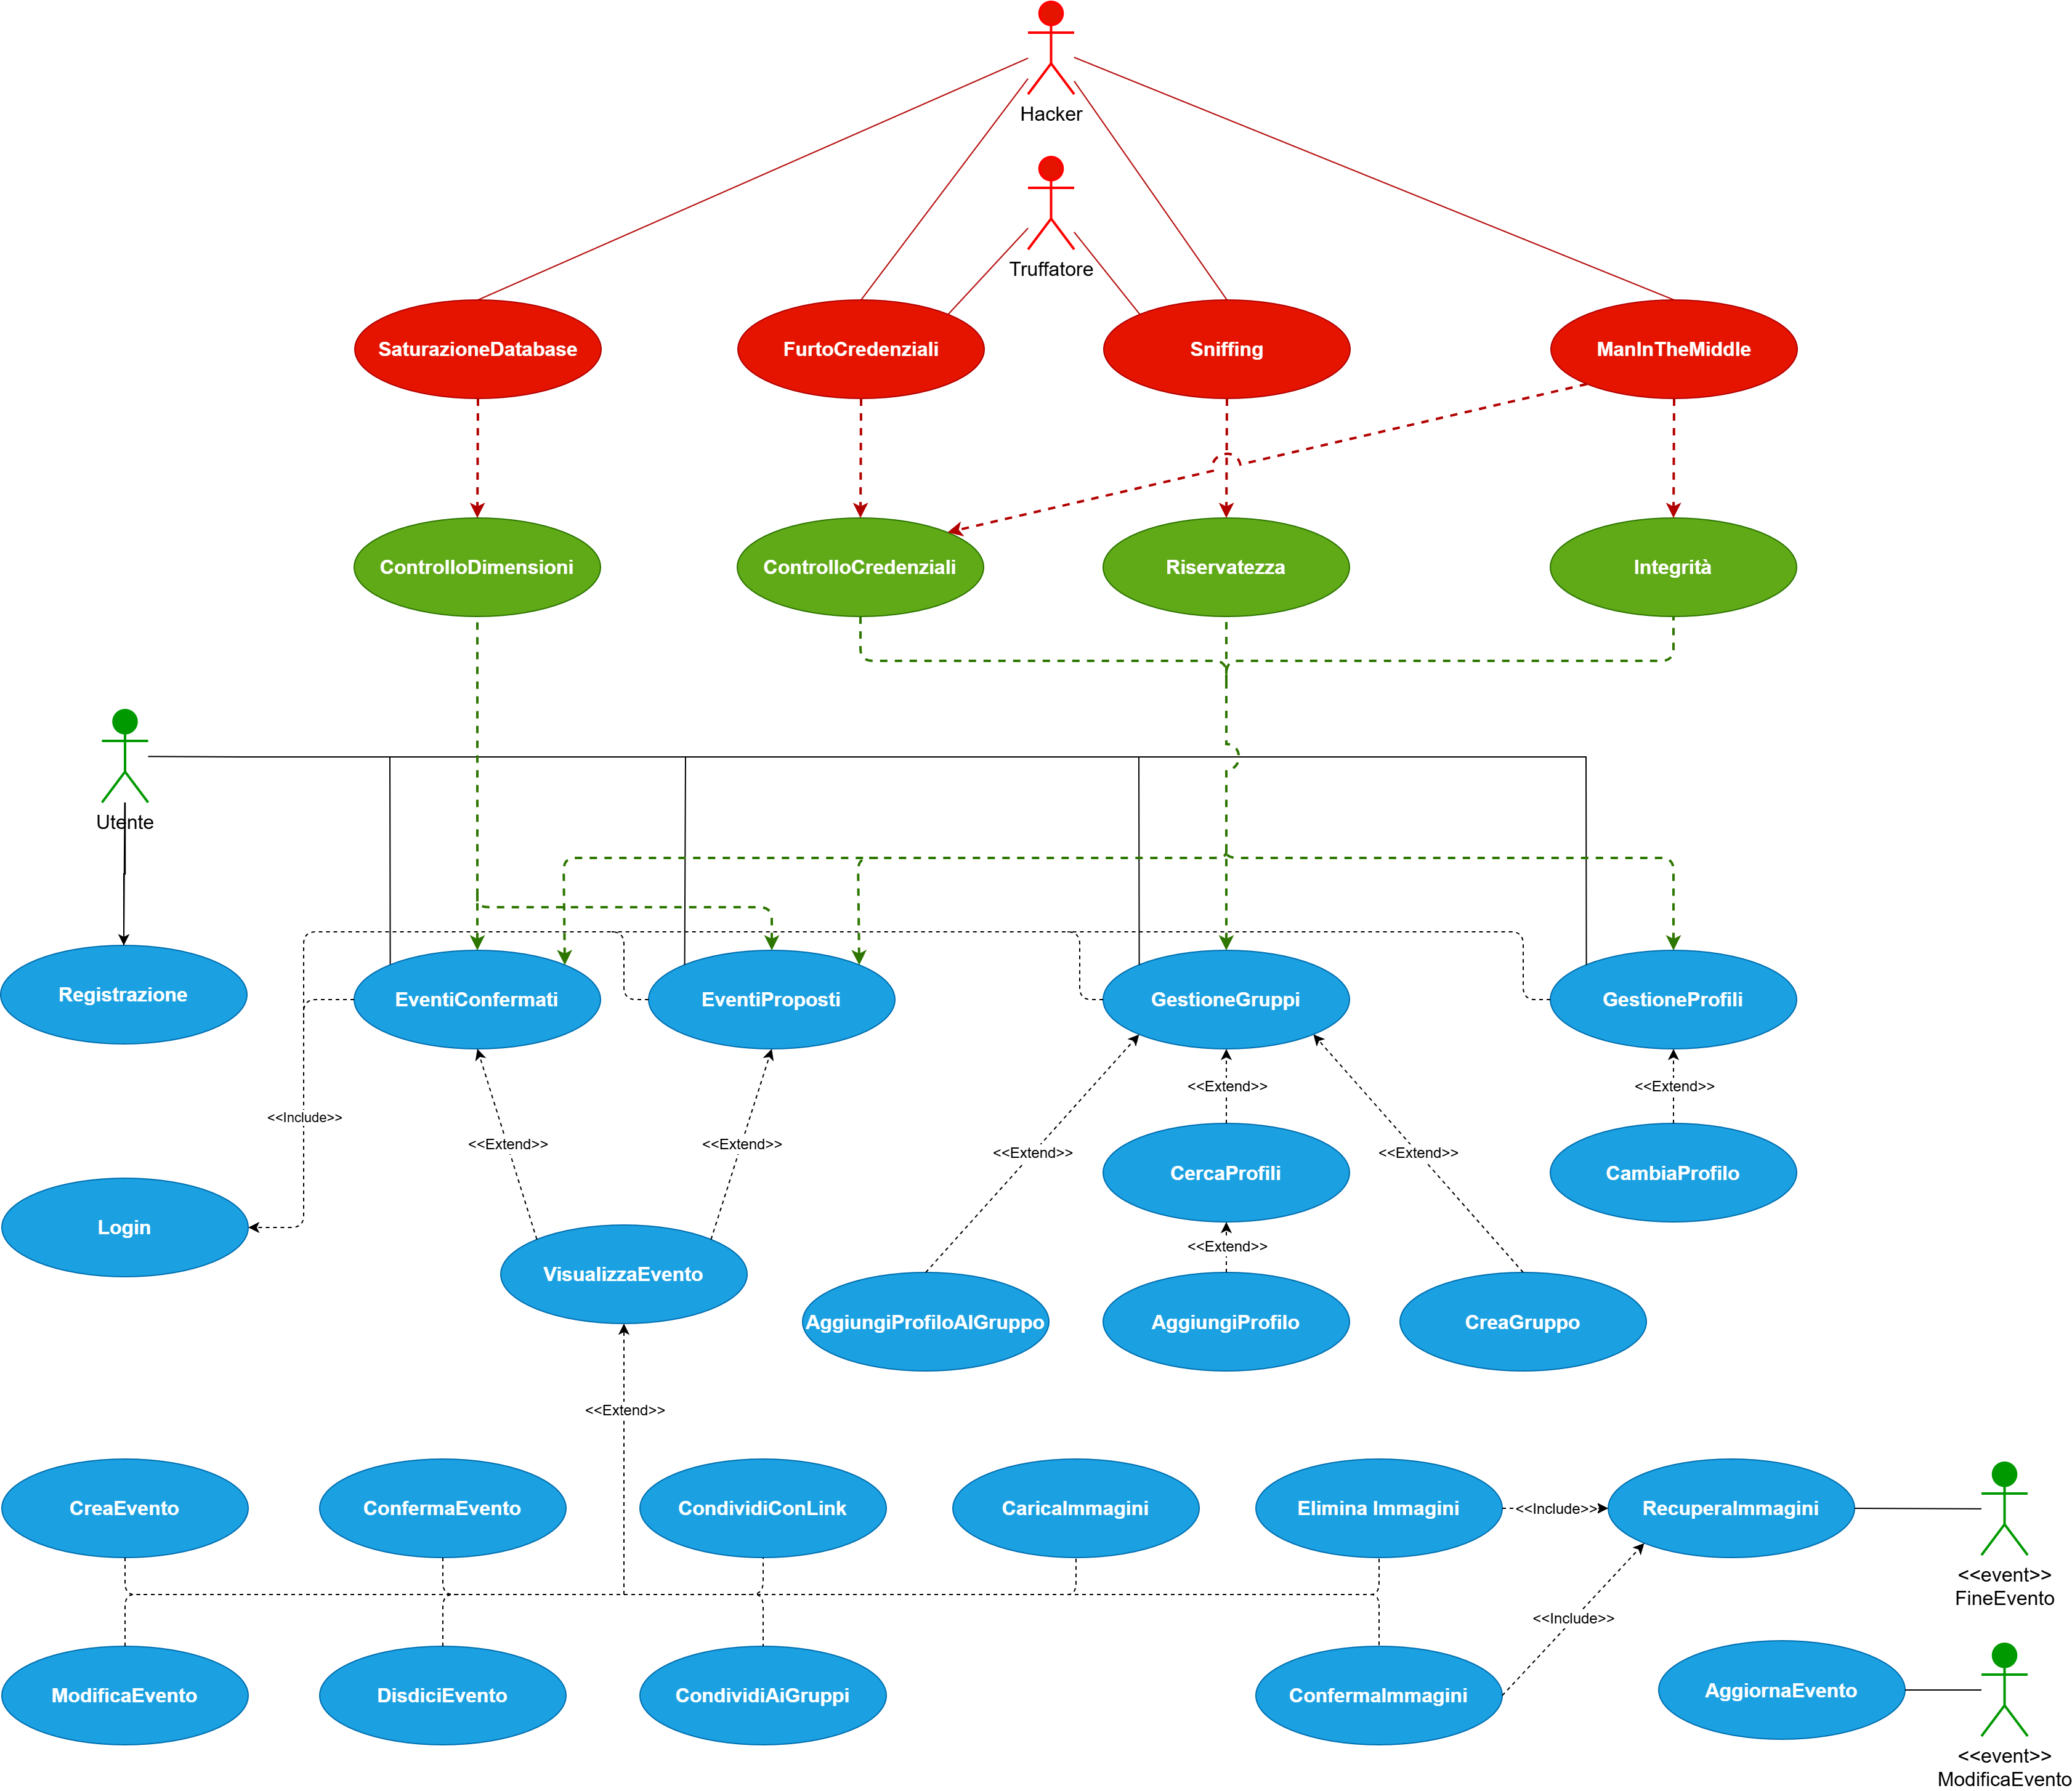
\includegraphics[width=\textwidth]{SecurityCase.png}
        \caption{Casi d'uso relativi alla sicurezza}
    \end{center}

\end{figure}
\clearpage

Visti i costi ed appurate le risorse a disposizione sono stati quindi identificati i seguenti requisiti
inerenti alla protezione dei dati e delle funzionalità di Wyd:
\begin{enumerate}
    \item Implementare un sistema di log per tracciare tutti i messaggi tra i client e i server, inclusi gli accessi, le richieste di prenotazione, di conferma, di sospensione e di invio e ricezione di dati
    \item I dati salvati devono essere protetti da un attaccante che abbia accesso al sistema, prendendo misure di sicurezza fisica, eventualmente cifrando i dati
    \item I dati inviati tra le parti remote devono essere protetti, utilizzando la cifratura dei dati
    \item Tutte le azioni avvenute sul sistema devono essere tracciate tramite un sistema di log.
    \item Il sistema deve essere resistente ad un alto numero di richieste contemporanee
    \item La dimensione delle richieste non deve superare una determinata soglia
\end{enumerate}

La visione e l'analisi dei log verrà gestita con uno strumento esterno, accessibile solo al personale autorizzato.


\begin{table}[htbp]
    \centering
    \begin{tabular} {|P{1.3cm}|P{11.2cm}|P{3cm}|}
        \hline
        \textbf{ID}             & \textbf{Requisiti}                                                                           & \textbf{Tipo}  \\
        \hline
        R21F                    & Implementazione di un sistema di log per tracciare tutti i messaggi
        tra i client e i server & Funzionale                                                                                                    \\
        \hline
        R22F                    & Le richieste non devono superare una certa dimensione                                        & Funzionale     \\
        \hline
        R7NF                    & I dati salvati devono essere protetti da un attaccante che abbia
        accesso al sistema, prendendo misure di sicurezza fisica, eventualmente
        cifrando i dati         & Non Funzionale                                                                                                \\
        \hline
        R8NF                    & I dati inviati tra le parti remote devono essere protetti, utilizzando la cifratura dei dati & Non Funzionale \\
        \hline
        R9NF                    & Il sistema deve essere resistente ad un alto numero di richieste contemporanee               & Non funzionale \\
        \hline
    \end{tabular}
    \caption{Requisiti di sicurezza}
\end{table}

\clearpage